\chapter{Emisi\'on de radio de una EAS}

\section{Mecanismos de emisi\'on}

	\subsection{Efecto Askaryan}
	
	\subsection{Interacci\'on con el campo geomagn\'etico}
	
	
	\begin{figure}[ht!]
		\centering
		\includegraphics[width=\textwidth]{./fig/EASRadio/geomComps_Malarge}
		\caption{\label{fig:geomComps_Malarge}
		asd
		}
	\end{figure}
	
	\begin{figure}[ht!]
		\centering
		\includegraphics[width=\textwidth]{./fig/EASRadio/geomComps_Tunka}
		\caption{\label{fig:geomComps_Tunka}
		asd
		}
	\end{figure}
	
\section{Se\~nal a nivel del suelo: Modelo de juguete}

	\subsection{EAS verticales}

	\subsection{EAS generadas por neutrinos ES}
	
	\begin{figure}[ht!]
		\centering
		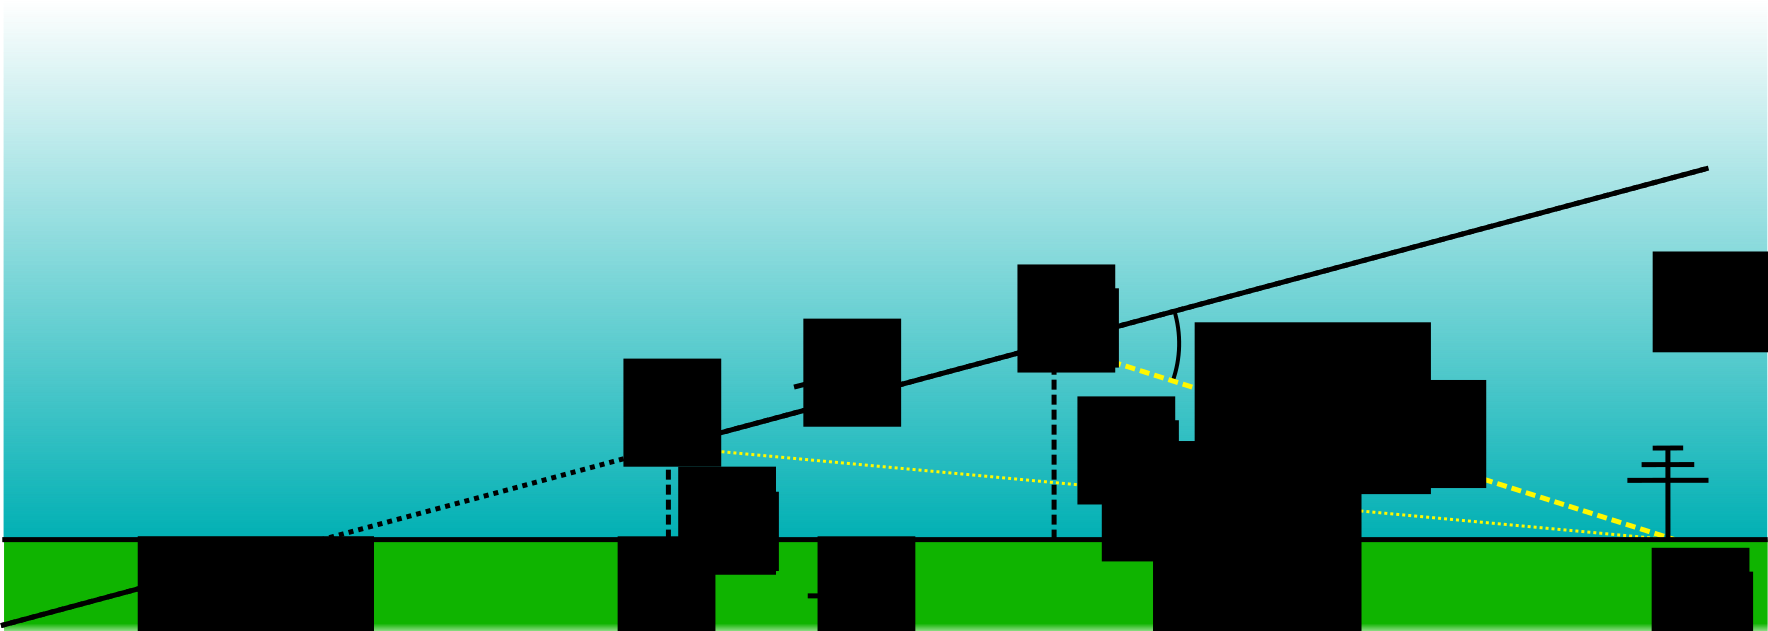
\includegraphics[width=0.95\textwidth]{./fig/EASRadio/timeDelaySchema}
		\caption{\label{fig:esRadio_schema}
		asd
		}
	\end{figure}
	
	\begin{equation}
	\begin{array}{rcl}
	\Delta t & = & \frac{1}{c}\left(l_e+nR-nd_{ref}\right) \\
	 & =  & 
	 \frac{1}{c}\left[l_e +
		n \sqrt{h_d^2+d_a^2+l_e^2+2h_dl_e \sin\theta - 2d_al_e\cos\theta} 
		-
		n \sqrt{h_d^2+d_a^2}
		\right]
	 
	\end{array}
	\end{equation}
	
	\begin{figure}[ht!]
		\centering
		\includegraphics[width=0.8\textwidth]{./fig/EASRadio/timeDelay_at}
		\caption{\label{fig:timeDelay_at}
		Tiempo de arrivo respecto de $d_{ref}/c$ como funci\'on del punto de emisi\'on a lo largo del eje de la lluvia. Los distintos colores representan antenas a diferentes distancias del punto de decaimiento del \tauon{} 
		}
	\end{figure}
	
	\begin{figure}[ht!]
		\centering
		\includegraphics[width=0.8\textwidth]{./fig/EASRadio/timeDelay_pd}
		\caption{\label{fig:timeDelay_pd}
		En linea punteada se muestra la distribuci\'on de part\'iculas a lo largo del eje de la lluvia. En linea llena se grafica el factor $1/R$ para antenas en diferentes posiciones.
		El campo el\'ectrico registrado en cada antena ser\'a proporcional al producto de estas funciones.
		}
	\end{figure}
	
	\begin{figure}[ht!]
		\centering
		\includegraphics[width=0.8\textwidth]{./fig/EASRadio/timeDelay_as}
		\caption{\label{fig:timeDelay_as}
		Se\~nal acumulada en funci\'on del tiempo obtenida a partir de 
		}
	\end{figure}
	
	\begin{figure}[ht!]
		\centering
		\includegraphics[width=0.8\textwidth]{./fig/EASRadio/timeDelay_spa}
		\caption{\label{fig:timeDelay_spa}
		M\'aximo de la se\~nal acumulada como funci\~non de la posici\'on de la antena.
		}
	\end{figure}
	
	